\documentclass[11pt,a4paper]{report}
\usepackage[cp1250]{inputenc}
\usepackage[english]{babel}
\usepackage[IL2]{fontenc}
\usepackage{amsmath}
\usepackage{amsfonts}
\usepackage{amssymb}
\usepackage{makeidx}
\usepackage{graphicx}
\usepackage{lmodern}
\usepackage{subfig}
\usepackage[autostyle]{csquotes}
\usepackage{setspace}
\usepackage[
backend=bibtex        % if we want unicode
,style=iso-authoryear % or iso-numeric for numeric citation method
,autolang=other       % to support multiple languages in bibliography      
]{biblatex}

\usepackage{titlesec}    
\titleformat{\chapter}[block]
{\normalfont\Large\bfseries}{\thechapter.}{1em}{\Large}
\titlespacing*{\chapter}{0pt}{-19pt}{19pt}


\titleformat{\section}[block]
{\normalfont\large\bfseries}{\thesection.}{1em}{\large}
\titlespacing*{\section}{0pt}{11pt}{19pt}


\usepackage{scrpage2}
\ifoot[]{}
\cfoot[]{}
\ofoot[\pagemark]{\pagemark}


\newcommand{\fakeparagraph}[1]{%
	\par\refstepcounter{paragraph}% Increase paragraph counter
	\paragraphmark{#1}% Add paragraph mark (header)
}



\graphicspath{ {./images/} }

\makeatletter
\def\blx@maxline{77}
\makeatother

\bibliography{Thesis.bib}

\newcommand*{\captionsource}[2]{%
	\caption[{#1}]{%
		#1%
		\\\hspace{\linewidth}%
		\textbf{Source:} #2%
	}%
}

\pagenumbering{gobble}

\usepackage[left=3.5cm,right=2cm,top=2cm,bottom=2cm]{geometry}
\author{Bc. Michal Koh�tek}
\title{Rozpozn�vanie emocion�lneho stavu pou��vate�a pomocou inteligentn�ch 
riadiacich syst�mov}
\begin{document}
	
\begin{titlepage}
	
{\centering
{\bfseries\LARGE UNIVERZITA KON�TANT�NA FILOZOFA V NITRE \par}
{\bfseries\LARGE FAKULTA PR�RODN�CH VIED \par}
\vfill
{\bfseries\LARGE ROZPOZN�VANIE EMOCION�LNEHO STAVU POU��VATE�A POMOCOU 
INTELIGENTN�CH RIADIACICH SYST�MOV\par}
\vspace{1cm}
{\bfseries\Large Diplomov� pr�ca\par}
\par}
\vfill
\Large{
�tudijn� program: Aplikovan� informatika (magistersk� II. St., denn�  
forma)\par
�tudijn� odbor:  AI15m - Aplikovan� informatika\par
�koliace pracovisko: Katedra Matematiky\par
�kolite�: Mgr. Martin Magdin, PhD\par}
\vfill
\textbf{Nitra 2018}\hfill\textbf{Bc. Michal Koh�tek}
\end{titlepage}
\onehalfspacing
\chapter*{Abstract}
\cfoot{}
Abstract goes here

\chapter*{Dedication}
To mum and dad

\chapter*{Declaration}
I declare that..

\chapter*{Acknowledgements}
I want to thank...

\tableofcontents
 
\chapter*{Introduction}
\pagenumbering{arabic}
\setcounter{page}{8}
\pagestyle{scrplain}
\begin{flushright}

"Smiles are probably the most underrated \\ facial expressions, 
 much more complicated \\ than most people realize. 
 There are dozens\\ of smiles, each differing in appearance \\
 and in the message expressed."\\
 - Paul Ekman
\end{flushright}

\paragraph{} Emotions are at the core of the human experience, albeit very hard 
to define, recognize and name, even in yourself. They are, by definition 
different from person to person, in diverse cultures and upbringings. Our 
perception of emotions and their classification has evolved in recent years. 
Various authors has tried to divide our emotional states into basic categories 
such as Ekman's Anger, Fear, Disgust, Happiness, Sadness and Surprise. However, 
recent work by psychologists and historians alike show, that a more complex 
look at emotions might be needed. 

\paragraph{}Emotional recognition changes with time. In 12th century, bards 
looked at yawning not as a sign of boredom or tiredness, but as a sign of a 
hidden and deep love. Early Christians recognized an emotion called "accidie", 
a lethargy and despair brought about by flying demons. Boredom, as such was 
first really  felt by the Victorians as a response to the new ideas of leisure 
time and self-improvement. Among the psychologist, there is a standing question 
whether some cultures feel some hard to define emotions more strongly, because 
they bothered to name them as separate kinds. For example the Russian "toska", 
a longing with nothing to long for, as coined by Vladimir Nabokov. Recent 
developments of cognitive science tell us, that emotions are not just simple 
reflexes, but inherently complex and elastic systems of response towards both 
the biologies 
that we've inherited and the cultures, that we live in now. They are not just 
simple chemistry, but a cognitive phenomena, not shaped only by our body 
functions, but also our thought process, concepts and language. The 
neuroscientist Lisa Feldman Barrett studies this 
dynamic relationship between words and emotions. She argues, that when a person 
learns a new word for an emotion, they also learn to feel and recognize it 
(\cite{barrett}). 
There is a historicity to emotions, they have changed in history, often times 
very dramatically, in response to new cultural expectations, religious beliefs, 
new ideas about gender, age, ethnicity, economical and political ideologies. 

\paragraph{}There is a push to increase our emotional intelligence. Emotions 
are so 
powerful, that in past, they were sometimes thought to be a cause of illness. 
In 17th century, there was a student attending the Swiss university in Basel. 
He 
came afflicted with fever, heart palpitations, skin sores on his body and was 
close to dying. When they sent him back home to die, he started getting better 
and by the time, he returned to his hometown, he almost entirely recovered. In 
1688, Johannes Hoffer, medical doctor, learnt of this case and 
many like it and coined the term for a severe homesickness as "nostalgia". Last 
confirmed death by nostalgia was an American soldier fighting during the First 
World War in France. In early 20th century, this feeling has morphed more into 
a longing for lost time, instead of homesickness and downgraded in severity. 
Nowadays, our culture celebrates happiness, as it is said to make 
us a better workers, parents and partners. However, in 16th century, this 
position was filled by sadness, as is evident by self-help books from that 
period, which tried to encourage sadness in readers by giving them lists of 
reasons to be disappointed.

\paragraph{}In order to study both basic emotions and their mixtures in the 
complex variety, we need appropriate detection and classification tools and 
techniques. Over the years, many psychologists and computer scientist 
collaborated to create a set of markers and techniques recognizing them. We 
will discuss several of them and compare their usefulness, reliability and 
practicality. These methods most often try to detect basic emotions such as the 
seven basic emotions (\cite{Ekman}) or a 12-point Affect Circumplex model 
(\cite{Russel}).
\begin{figure} [ht]
	\centering
	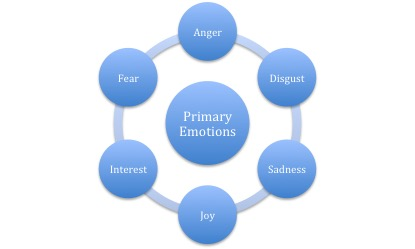
\includegraphics{images/Primary_Emotions}
	\caption{Six primary emotions}
	\label{fig:}
\end{figure} 




\chapter{Emotion classification} \paragraph{}Emotion classification is a 
contested issue in 
emotion research and in affective science. The two fundamental viewpoints of 
affective scientists' approach are: \begin{enumerate}
	\item Emotions as discrete and fundamentally different constructs
	\item Emotions as fluid and characterized on a dimensional basis in 
	groupings
\end{enumerate}
Various categorizations of emotions also vary in description how emotions 
relate to each other.
\section{Discrete models of emotions}
\paragraph{}Discrete emotion theory claims that there is a small 
number 
of core affects. 
This number can vary depending on the proponent, for example Silvan Tomkins 
considered nine basic emotions. Six, that came evolutionarily earlier, 
interest-excitement, enjoyment-joy, surprise-startle, distress-anguish, 
anger-rage, fear-terror, once that evolved later, shame-humiliation and finally 
disgust and dissmell, which he later took back. In the paired affects, the 
first of the pair is the mild manifestation and the second the more intense. 
(\cite{tomkins1962affect}), (\cite{tomkins1963affect}). This model is somewhat 
controversial nowadays among affective theorists, especially over Tomkins' firm 
insistence that there were nine and only nine, biologically based affects. He 
also argued, that these affects are quite discreet (in contrast to the more 
muddled and complex emotions) and that they shared a common biological heritage 
with what Darwin called emotions in animals (\cite{darwin1998expression}). They 
also differ from Freudian drives in lacking an object.
\paragraph{}Similarly, Carroll Izard delineated 12 discrete emotions: 
interest, joy, surprise, sadness, anger, disgust, contempt, self-hostility, 
fear, shame, shyness and guild. He measured these via his Differential Emotion 
Scale (\cite{Izard}). Among other contributors to this theory, such as John 
Watson, Edwin Newman and Ross Buck, Paul Ekman performed a series of 
cross-cultural studies with Carrol Izard and reported that there are at least 
six emotions, that people across the world produce and are able to recognize. 
This was further evidenced when researchers approached the people of New Guinea 
with no previous exposure to Westerners nor their culture. When they showed 
them pictures of people expressing six core emotions, subjects could in fact 
point out the different emotions and distinguish between them 
(\cite{ekmanguinea}). 

\section{Dimensional models of emotions}
\paragraph{} There are various theoretical and practical reasons for which some 
researchers define emotions according to one or more dimensions. Dimensional 
models are an attempt to conceptualize human emotions by defining where they 
lie in two or three dimensions. Most incorporate valence and arousal or 
intensity dimensions. In contrast to theories of basic emotion, which propose 
that different emotions arise from separate neural systems, dimensional models 
suggest that a common and interconnected neurophysiological system is 
responsible for all affective states. (\cite{posner}) 
\paragraph{}In 1897, Wilhelm Max Wundt proposed, that emotions can be described 
by three dimensions: 
"pleasurable versus unpleasurable", "arousing versus subduing" and "strain 
versus relaxation" (\cite{wundt2017outlines}). Later, Harold Schlosberg named 
three dimension, "pleasantness�unpleasantness", "attention�rejection" and 
"level of activation" (\cite{schlosberg1954three}).
\paragraph{}Another model, called the circumplex model, was developed by James 
Russell. This model suggest that emotions are distributed in a two-dimensional 
circular space, containing both arousal and valence dimensions. The vertical 
axis represents arousal, horizontal axis valence and the center of the circle 
represents a neutral valence and medium level of arousal.(\cite{circumplex}).

\begin{figure} [ht]
	\centering
	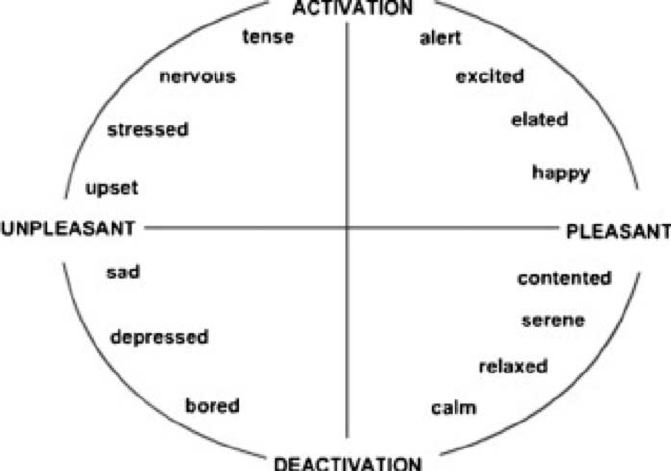
\includegraphics[scale=0.4]{images/russel_model}
	\centering
	\caption{ A. Russell�s (1980) circumplex model of affect}
	\label{fig:}
\end{figure} 

This model was later modified by Russel and Lisa Feldman Barret, which they 
described as representative of core affect, which are the most elementary 
feelings that need not be directed toward anything. Different prototypical 
emotional episodes, or clear emotions that are evoked or directed by specific 
objects, can be plotted on the circumplex, according to their levels of arousal 
and pleasure (\cite{Russell1999CoreAP}).

\paragraph{}Another model of emotion appeared in 1992. This two-dimensional 
model consists of vectors, that point in two directions. The vector model 
assumes that there is always an underlying arousal dimension and that valence 
determines the direction in which a particular emotion lies.
\begin{figure}
		\centering
		\subfloat[2D
		representation]{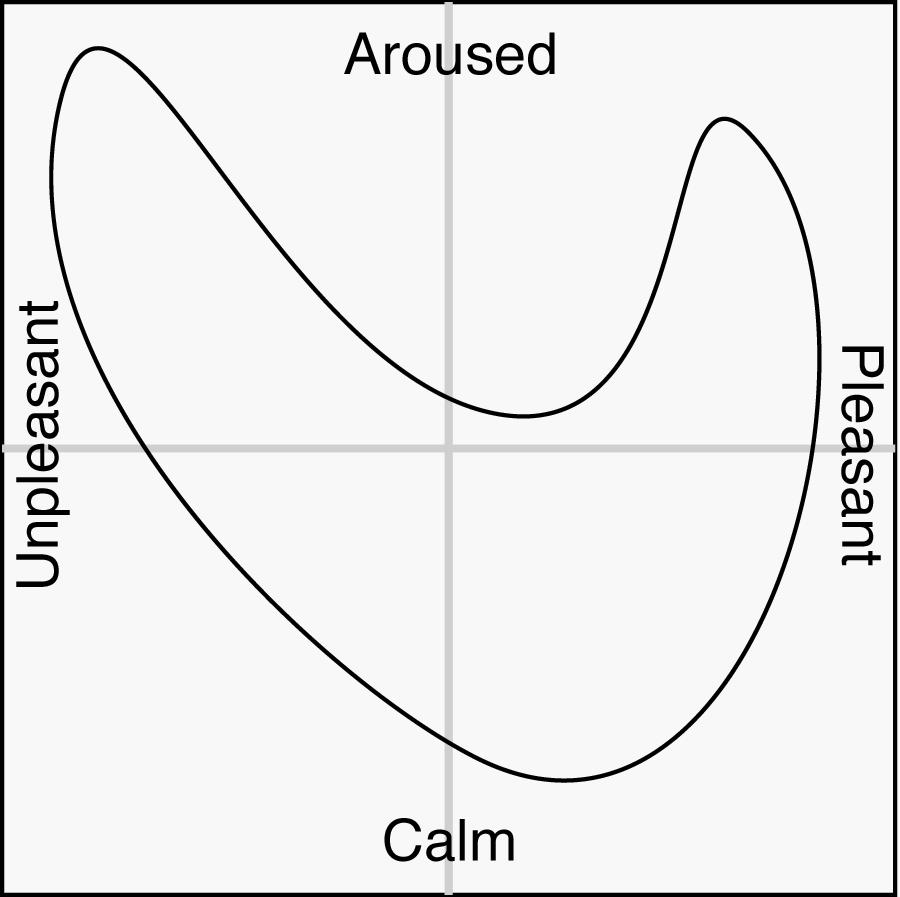
\includegraphics[width=0.2\linewidth]{images/vector0}}%
		\qquad
		\subfloat[3D 
		representation]{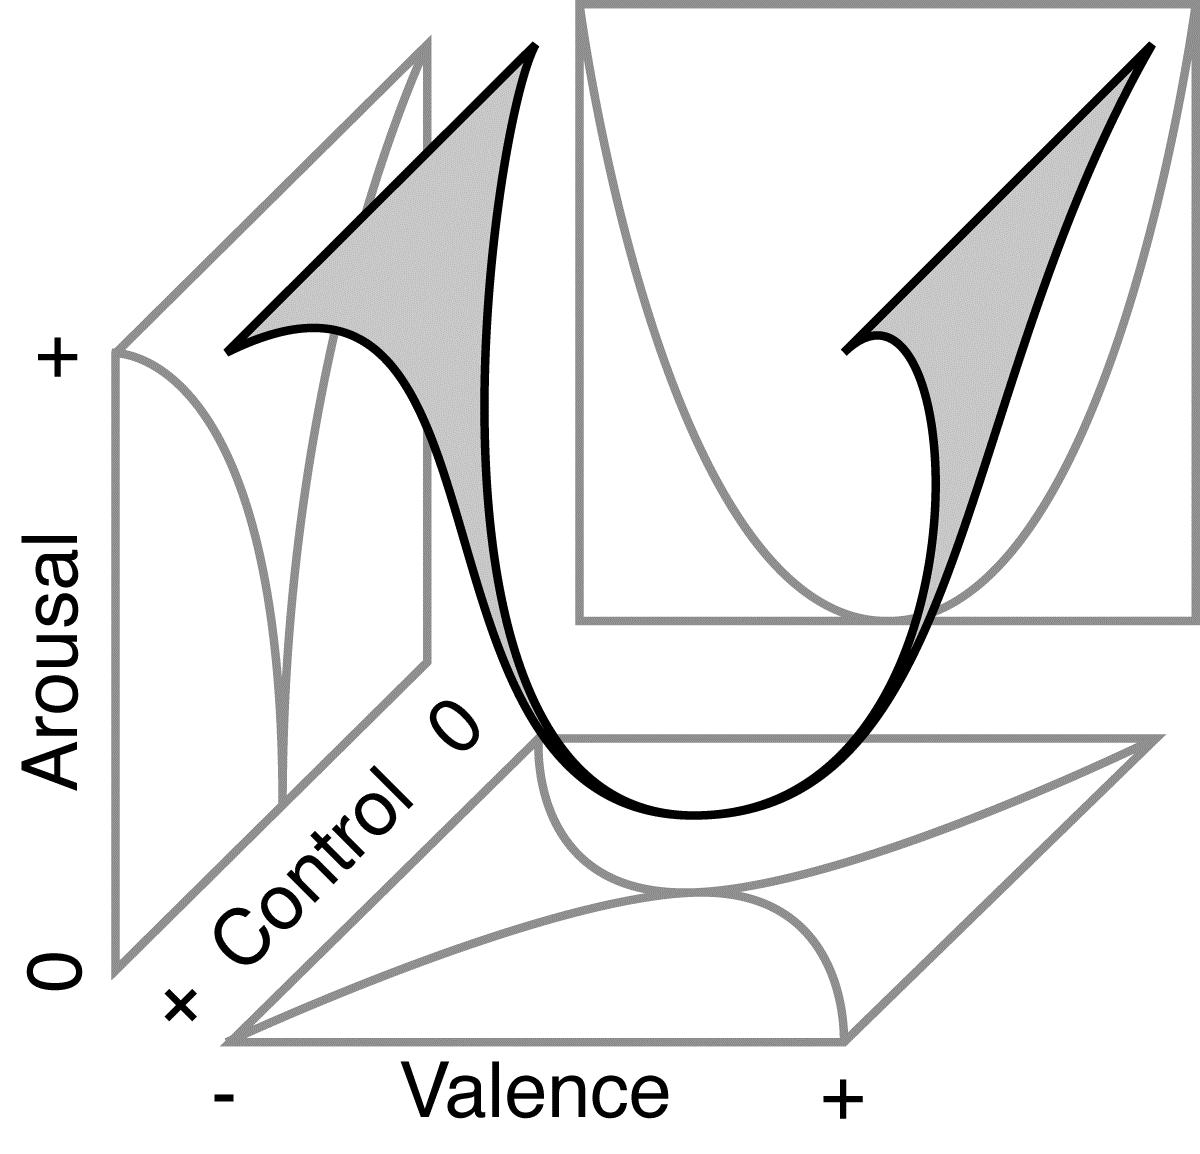
\includegraphics[width=0.2\linewidth]{images/vector1}}%
		\caption{Vector model of emotions}
		\label{fig:}
\end{figure}

\paragraph{} The positive activation � negative activation (PANA) was 
originally created in 1985 by David Watson and Auke Tellegen. It suggests that 
positive and negative affect are two separate systems. Like in the vector 
model, states of higher arousal tend to be defined by their valence and states 
of lower arousal tend to be more neutral in term of valence. In the PANA model, 
the vertical axis represents low to high positive affect and the horizontal 
axis represents low to high negative affect. The dimensions of valence and 
arousal lay at a 45-degree rotation over these axes (\cite{watson}).

\begin{figure} [ht]
	\centering
	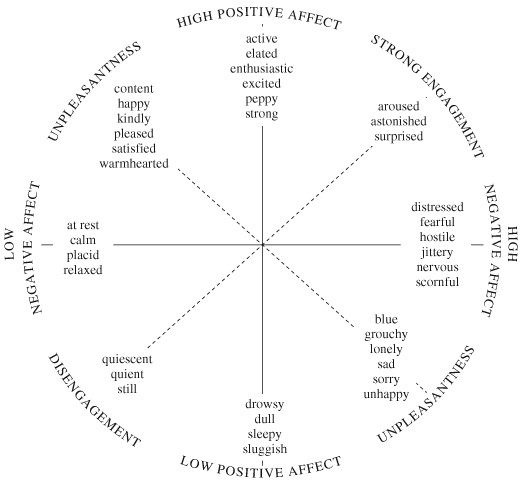
\includegraphics[scale=0.4]{images/consensual}
	\centering
	\caption{Consensual (PANA) model of emotion}
	\label{fig:}
\end{figure}

\paragraph{} In 1980, Robert Plutchik constructed a wheel of emotions. This 
model is a hybrid of both basic-complex categories and dimensional theories. 
Emotions are arranged in concentric circles, with the more basic emotions on 
the inner circles, while the outer circles are occupied by complex emotions.  
Notably, outer circles are also formed by blending the inner circle emotions. 
Plutchik suggested 8 primary contrasting pairs of emotions. Joy/sadness, 
anger/fear, trust/disgust and surprise/anticipation. Like colors, primary 
emotions can be expressed at different intensities and can mix with one another 
to form different emotions (\cite{Plutchik1988}).

\begin{figure} [ht]
	\centering
	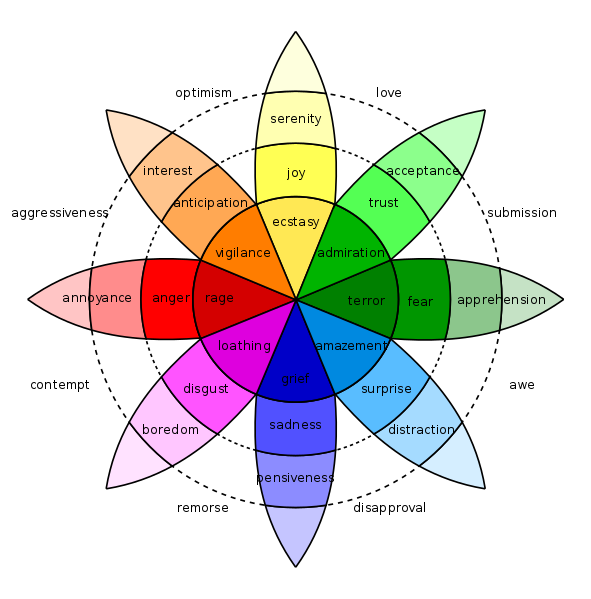
\includegraphics[scale=0.3]{images/Plutchik_wheel}
	\centering
	\caption{Plutchik's wheel of emotions}
	\label{fig:}
\end{figure}

\paragraph{} The PAD emotional state model was developed by Albert Mehrabian 
and James A. Russel. It uses three numerical dimensions, \textbf{P}leasure, 
\textbf{A}rousal, and \textbf{D}ominance to represent all emotions 
(\cite{mehrabian1980basic}). Initially it's use was in a theory of 
environmental psychology, the core idea being that physical environments 
influence people through their emotional impact (\cite{mehrabian1974approach}). 
Subsequently it was used by Peter Lang to propose a physiological theory of 
emotion (\cite{lang}). Furthermore, it was also used by Russel to develop a 
theory of emotional episodes (\cite{coreaffect}). The Pleasure-Displeasure 
Scale measures how pleasant an emotion may be. Anger and fear are, for 
instance, unpleasant emotions and thus score high on the displeasure. 
Contrarily, joy is a pleasant emotion. The Arousal-Nonarousal Scale measures 
the intensity of emotion. For instance while both anger and rage are unpleasant 
emotions, rage is much more intense than anger. Boredom, while also an 
unpleasant state, has a low arousal volume. Lastly, the 
Dominance-Submissiveness Scale shows the dominant nature of the emotion. While 
both fear and anger are unpleasant emotions, anger is dominant, but fear is a 
submissive emotion (\cite{mehrabian1980basic}).
\begin{figure} [ht]
	\centering
	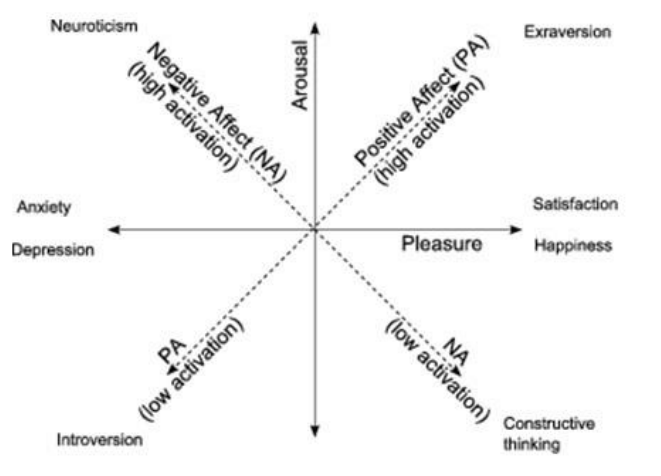
\includegraphics[scale=0.4]{images/pad_model}
	\centering
	\caption{PAD emotional state model}
	\label{fig:}
\end{figure}
A more abbreviated version of the PAD model has also been used in 
organizational studies where the emotions towards specific entities or products 
are measured. It uses just 4 values for each dimension, providing only 64 
values for emotions (\cite{abbrpad}). 

\paragraph{} An example of three-dimensional models, the L�vheim cube of 
emotion was presented where the signal substances (dopamine, noradrenaline and 
serotonin) form the axes of a coordinate system, and the eight basic emotions 
according to Tomkins are placed in the eight corners.
\begin{figure} [ht]
	\centering
	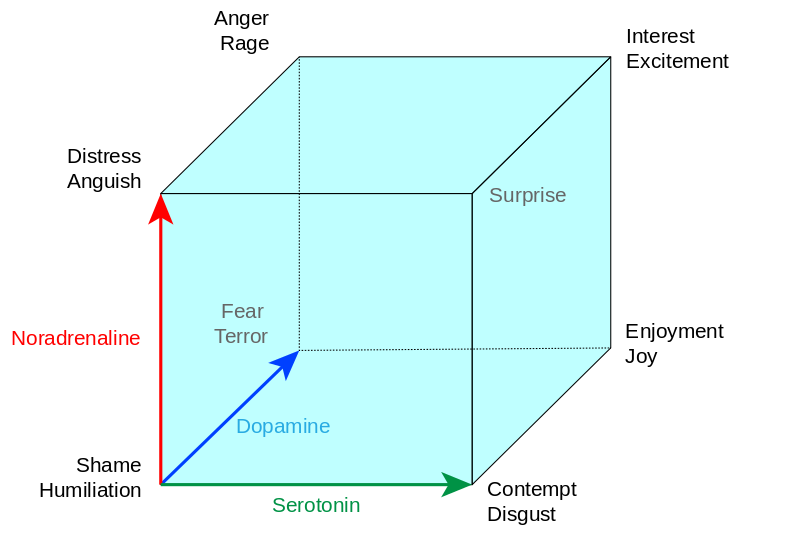
\includegraphics[scale=0.4]{images/lovheimcube}
	\centering
	\caption{L�vheim cube of emotion}
	\label{fig:}
\end{figure}
As shown on the figure below, anger is produced by the combination of low 
serotonin, high dopamine and high noradrenaline. Conversely joy is a product of 
high serotonin, high dopamine and low noradrenaline. Since none of the axis is 
identical to valence \footnote{pleasantness}, the cube seems somewhat rotated 
when 
compared to other models (\cite{Lvheim2012ANT}).


\paragraph{} Most recently Cowen and Kelter, researchers from University of 
California, Berkeley introduced a statistically derived taxonomy of emotion. 
(\cite{Cowen201702247}) \blockquote{Across self-report methods, we find that 
the [2185] 
videos [selected and shown to volunteer subjects] reliably elicit 27 distinct 
varieties of reported emotional experience. Further analyses revealed that 
categorical labels such as amusement better capture reports of subjective 
experience than commonly measured affective dimensions (e.g., valence and 
arousal). Although reported emotional experiences are represented within a 
semantic space best captured by categorical labels, the boundaries between 
categories of emotion are fuzzy rather than discrete. By analyzing the 
distribution of reported emotional states we uncover gradients of emotion�from 
anxiety to fear to horror to disgust, calmness to aesthetic appreciation to 
awe, and others�that correspond to smooth variation in affective dimensions 
such as valence and dominance. Reported emotional states occupy a complex, 
high-dimensional categorical space} 

\paragraph{}More dimensional models of emotion have been developed, though 
there are just a few that remain as the dominant models currently accepted by 
most (\cite{comparison}). There have been observed great cultural differences 
in the way in which emotions are valued, expressed and regulated. The social 
norms for emotions, like the frequency with or circumstances in which they are 
expressed also vary drastically in diverse cultures. An important piece of 
evidence that disputes the universality of emotions is language. Emotions such 
as the schadenfreude \footnote{The experience of pleasure, joy, or 
self-satisfaction that comes from learning of or witnessing the troubles, 
failures, or humiliation of another.} in German and saudade\footnote{Deep 
emotional state of nostalgic or profound melancholic longing for an absent 
something or someone that one loves.} in Portuguese are commonly expressed in 
emotions in their respective languages, but lack an English equivalent. Thus it 
is reasonable in our research to scale back on the complex, culturally 
influenced emotions and focus on the more primal, basic emotions, that may be 
more quantifiable by studying the physiological markers and responses in 
subjects.
\section{Physiological responses of emotions}
%\paragraph{}When dealing with physiological effects of emotion, we come across 
%a few prevalent theories. The James-Lange theory is one of the earliest 
%theories of emotion within modern psychology. It was developed independently 
%by 
%William James and Carl Lange in 19th century. The basic premise 
%\footnote{Which 
%is also the point of most criticism} is that physiological arousal instigates 
%the experience of emotion, i.e., the arousal precedes and causes the emotion 
%(\cite{walter}). According to the Cannon-Bard theory of emotions, the emotion 
%is accompanied by physiological arousal.


\paragraph{} In order for us to be able to detect and recognize emotions from 
the data samples, we need to asses which physiological effects of emotions we 
want to capture. Therefore, we need to divide our standard basic emotions 
depending on the combination of kinds and intensity of effects they have on 
human body. There is a difficulty with dealing with physiological markers of 
emotions in that not all emotions do perceivably alter the physiology of the 
subjects. That is the reason, why we need to supplement this data with the 
facial expressions or, as we have tried to confirm, ocular movements. 

\paragraph{} Anger is one of the emotions with more pronounced physiological 
signs. It comes along with faster and deeper breathing 
(\cite{respiratoryfeedback}), increased heart rate, blood pressure, 
perspiration and tensing of muscles. Fear, on the other hand, shares most of 
the surface physiological marks with anger, such as the accelerating breathing 
rate, heart rate and muscle tension, but facial expression and body language 
are vastly different. Even deeper markers, like the cortisol levels differ 
after subjecting a person to these stressors (\cite{Moons2010AngerAF}). Joy, 
sadness, disgust and surprise are similar to each other in their difficulty to 
asses using pure physiological markers and therefore requiring additional 
information, usually in form of facial expression.

\section{Current approaches in detecting and classifying emotions}
\paragraph{}As we've described motion recognition is an important object of 
studies in today's 
psychology, with many potential uses and applications. Correctly assessing and 
recognizing subject's emotion can lead to better understanding it's motivation 
and inner working. Data gained through methods described below can be used to 
assess the effectiveness of marketing, comprehensibility of lectures, usability 
of user interfaces, measure of impact of psychological therapy, etc. Previous 
implementations of emotion recognition technology often have had a multitude of 
disadvantages, which prohibited it's daily and widespread usage. Therefore, we 
have set upon creating a solution, that is modular, reasonable to wear for 
prolonged durations of time and still maintains a degree of reliability in 
captured data. We can do so by using an array of data resources, that 
complement each other, diminishing their disadvantages and reinforcing 
confidence.

\paragraph{}One particularly rich resource for data on human emotions is the 
brain. In 2015 a group of researchers in India published a paper on a system 
using EEG signals as input, Independent Component Analysis \footnote{A 
statistical procedure used for splitting up a set of mixed signals into its 
sources}, Kernel Destiny Estimation \footnote{A method used for feature 
extraction of signals by computing density estimate using kernel-smoothing 
method} and an Artificial Neural Network to  transform the inputs into 
meaningful outputs. They observed better results for clustering of EEG and ECG 
data stream (\cite{LAHANE2015574}). Similar approach was taken by researchers 
in China. Main difference in their approach is that they first applied EMD 
\footnote{Empirical Mode Decomposition} strategy to split EEG signals into a 
series of intrinsic mode functions, which were then fed as sample entropies and 
as feature vectors into SVN\footnote{Support Vector Machine} classifier for 
testing and training. With this approach, they claim to have reached accuracy 
levels of 94.98\% for binary-class tasks and  93.20\% for the multi-class task 
on DEAP database (\cite{zhang}).  Also in 2016, researchers from the Duke 
University, North Carolina demonstrated an emotional recognition technique 
using functional MRI with results, that brain-based models may, in future, 
allow us deeper understanding and assessing emotional status in clinical 
settings, particularly in individuals incapable of providing self-report of 
their own emotional experience (\cite{kragel}). These techniques are, however, 
impossible to replicate on greater scale and in the context of a classroom, or 
other commonplace environment.

\paragraph{}Another indicator of the subject's emotional state is heartbeat. 
Research published in May 2013 in International Journal of Engineering Trends 
and Technology shown compelling data gathering by means of 
ECG\footnote{Electrocardiography} and shown 
differences in ECG signal in subjects in chosen emotional states. 
\footnote{This study was limited to joy, sadness, fear and anger} 
(\cite{shalini2013emotion}). More complex approach was taken by researchers at 
University of Calabria in collaboration with Washington State University. 
Instead of applying a single or a few sensors to study physiological states, 
they used a whole BSN\footnote{Body Sensor Network, specialized Wireless Sensor 
Network applied to the whole human body.} Such networks can include 
accelerometers, gyroscopes, pressure sensors for body movements
and applied forces, skin/chest electrodes (for electrocardiogram
(ECG), electromyogram (EMG), galvanic skin response (GSR), and
electrical impedance plethysmography (EIP)), (PPG) sensors, microphones (for 
voice, ambient, and heart sounds), scalp-placed electrodes for 
electroencephalogram (EEG) (\cite{gravina}). Albeit they were not focusing 
primarily on emotion recognition, this survey shows consequential advancement 
in the state-of-the-art body data collection, especially in the data fusion 
techniques. Similar approach using a variety of sensors and data sources was 
also taken by \cite{MOSCIANO201748} to reasonably accurately classify the two 
dimensions of affect both normal and simulated critical working conditions.

\paragraph{}An interesting approach to emotion detection and classification is 
based upon speech patterns and variations and are better suited for emotions, 
which are otherwise hard to physiologically measure, such as sadness and joy. 
One study shows, that speech signal and feature distances of letters and words 
vary depending on the mood and emotional state of the subject. The study was 
done upon the sample size of 30 people, however, researchers point out, that 
for getting better accuracy, one should consider the data collected from one 
person rather than considering the data from a group of people 
(\cite{DAVLETCHAROVA201591}).

\paragraph{}In terms of evaluating arousal, respiration-based emotion 
recognition shows promise. A study in China showed, that using respiration data 
to evaluate valence and arousal levels of Russel theory, they reached 
classification accuracy of valence and arousal at 73.06\% and 80.78\%, 
respectively (\cite{zhang2}). When compared to other studies using ECG or 
EEG data, the accuracy of valence levels are not exceptional, however the 
classification accuracy of arousal better than most other approaches.

\paragraph{}A study on thermal behavior of anger, disgust, fear, joy and 
sadness was carried out in 2016. When an emotion occurs a change in facial 
temperature appears due to the blood flow that the body emits through blood
vessels in the subcutaneous area (\cite{stephanos}). For example, research 
focused on the emotion of joy, in other words, when a subject is smiling, it has
been found that the temperature of the nose and forehead
decreases during this event (\cite{SALAZARLOPEZ2015149}). Biomedical thermal 
images of the facial
expressions of 44 subjects were captured experiencing the five studied 
emotions, with results of this test at 89.9\% success rate (\cite{Albarran}).

\paragraph{}Another novel approach was experimented with by researchers from 
American University of Sharjah, United Arab Emirates. They have created a 
software touch keyboard, that was installed on Android smartphones, which then 
have been collecting sensor data while users were typing on the keyboard. As 
they have been typing, he or she were prompted to indicate their current 
emotional state, which then tagged the sensor data collected for the particular 
user. Afterwards the data was classified by multiple machine learning 
algorithms to find the best classification method. Based on 
ROC\footnote{Receiver Operating Characteristic} and Precision-Recall curves, it 
was concluded that both J48 and Multi-response linear regression performed
well. This system demonstrates that it is possible to enable emotion 
recognition on mobile phones using built-in sensors (\cite{ZUALKERNAN20171}). 
More research is, nevertheless, needed to precisely ascertain the accuracy and 
applicability of such solution in common practice.

\paragraph{}One approach seems to be very promising, especially due to it's 
implementation in commercial solutions and services. That approach is based on 
facial expression evaluation and it is used by a wide variety of software 
vendors and research institutions. One such research has used Microsoft Kinect 
for 3D face modeling with a goal to computationally recognize facial 
expressions of seven basic emotional states: neutral, joy, surprise, anger, 
sadness, fear and disgust. The subjects of the experiment were six men aged 
26-50 years, told to mimic expressions shown on the screen. Researchers  used 
nearest neighbor classifier (3-NN) and two-layer neural network classifier (MLP)
with 7 neurons in the hidden layer with output accuracy rate of 96\% for 
random division of data and 73\% for "natural" division of data 
(\cite{TARNOWSKI20171175}).
%mention affectiva and other commercial sdk and api
\subsection{Emotion recognition APIs and SDKs used in commercial environment}

\paragraph{}There are two questions, that remains unanswered. Is our current 
method of selecting impulses the correct one? Are we rating approaches the 
right way? In research mentioned above, there are mainly two types of 
referential data. One is based on self-identifying emotions, the other on using 
previously assorted categories of pictures or impulses. As we've mentioned 
before, self-identifying emotions is a hard task for most people and it is the 
task, that we aim to solve. Also, is the methodology we use, to personally 
evaluate emotions the correct one? We usually refer to the previous 
evaluations, that trace back to psychologist and we take their emotion 
assessments at face value. It might be wise, that we should ignore previous 
results and rather try to classify and categorize emotions from ground up and 
later compare them with historical data. Finally, most of the researches 
delving into face expression-based emotion recognition declare their statistics 
based upon the success rate of recognizing simple expressions, not emotions 
themselves.

\chapter{Data gathering methodology}
\section{Hardware}
\section{Software}

\chapter{Data evaluation}

\chapter{Results}
\printbibliography
\end{document}